\documentclass[]{book}
\usepackage{lmodern}
\usepackage{amssymb,amsmath}
\usepackage{ifxetex,ifluatex}
\usepackage{fixltx2e} % provides \textsubscript
\ifnum 0\ifxetex 1\fi\ifluatex 1\fi=0 % if pdftex
  \usepackage[T1]{fontenc}
  \usepackage[utf8]{inputenc}
\else % if luatex or xelatex
  \ifxetex
    \usepackage{mathspec}
  \else
    \usepackage{fontspec}
  \fi
  \defaultfontfeatures{Ligatures=TeX,Scale=MatchLowercase}
\fi
% use upquote if available, for straight quotes in verbatim environments
\IfFileExists{upquote.sty}{\usepackage{upquote}}{}
% use microtype if available
\IfFileExists{microtype.sty}{%
\usepackage{microtype}
\UseMicrotypeSet[protrusion]{basicmath} % disable protrusion for tt fonts
}{}
\usepackage[margin=1in]{geometry}
\usepackage{hyperref}
\hypersetup{unicode=true,
            pdftitle={Econometrics with R at SciencesPo},
            pdfauthor={Florian Oswald and Jean-Marc Robin},
            pdfborder={0 0 0},
            breaklinks=true}
\urlstyle{same}  % don't use monospace font for urls
\usepackage{natbib}
\bibliographystyle{apalike}
\usepackage{color}
\usepackage{fancyvrb}
\newcommand{\VerbBar}{|}
\newcommand{\VERB}{\Verb[commandchars=\\\{\}]}
\DefineVerbatimEnvironment{Highlighting}{Verbatim}{commandchars=\\\{\}}
% Add ',fontsize=\small' for more characters per line
\usepackage{framed}
\definecolor{shadecolor}{RGB}{248,248,248}
\newenvironment{Shaded}{\begin{snugshade}}{\end{snugshade}}
\newcommand{\KeywordTok}[1]{\textcolor[rgb]{0.13,0.29,0.53}{\textbf{#1}}}
\newcommand{\DataTypeTok}[1]{\textcolor[rgb]{0.13,0.29,0.53}{#1}}
\newcommand{\DecValTok}[1]{\textcolor[rgb]{0.00,0.00,0.81}{#1}}
\newcommand{\BaseNTok}[1]{\textcolor[rgb]{0.00,0.00,0.81}{#1}}
\newcommand{\FloatTok}[1]{\textcolor[rgb]{0.00,0.00,0.81}{#1}}
\newcommand{\ConstantTok}[1]{\textcolor[rgb]{0.00,0.00,0.00}{#1}}
\newcommand{\CharTok}[1]{\textcolor[rgb]{0.31,0.60,0.02}{#1}}
\newcommand{\SpecialCharTok}[1]{\textcolor[rgb]{0.00,0.00,0.00}{#1}}
\newcommand{\StringTok}[1]{\textcolor[rgb]{0.31,0.60,0.02}{#1}}
\newcommand{\VerbatimStringTok}[1]{\textcolor[rgb]{0.31,0.60,0.02}{#1}}
\newcommand{\SpecialStringTok}[1]{\textcolor[rgb]{0.31,0.60,0.02}{#1}}
\newcommand{\ImportTok}[1]{#1}
\newcommand{\CommentTok}[1]{\textcolor[rgb]{0.56,0.35,0.01}{\textit{#1}}}
\newcommand{\DocumentationTok}[1]{\textcolor[rgb]{0.56,0.35,0.01}{\textbf{\textit{#1}}}}
\newcommand{\AnnotationTok}[1]{\textcolor[rgb]{0.56,0.35,0.01}{\textbf{\textit{#1}}}}
\newcommand{\CommentVarTok}[1]{\textcolor[rgb]{0.56,0.35,0.01}{\textbf{\textit{#1}}}}
\newcommand{\OtherTok}[1]{\textcolor[rgb]{0.56,0.35,0.01}{#1}}
\newcommand{\FunctionTok}[1]{\textcolor[rgb]{0.00,0.00,0.00}{#1}}
\newcommand{\VariableTok}[1]{\textcolor[rgb]{0.00,0.00,0.00}{#1}}
\newcommand{\ControlFlowTok}[1]{\textcolor[rgb]{0.13,0.29,0.53}{\textbf{#1}}}
\newcommand{\OperatorTok}[1]{\textcolor[rgb]{0.81,0.36,0.00}{\textbf{#1}}}
\newcommand{\BuiltInTok}[1]{#1}
\newcommand{\ExtensionTok}[1]{#1}
\newcommand{\PreprocessorTok}[1]{\textcolor[rgb]{0.56,0.35,0.01}{\textit{#1}}}
\newcommand{\AttributeTok}[1]{\textcolor[rgb]{0.77,0.63,0.00}{#1}}
\newcommand{\RegionMarkerTok}[1]{#1}
\newcommand{\InformationTok}[1]{\textcolor[rgb]{0.56,0.35,0.01}{\textbf{\textit{#1}}}}
\newcommand{\WarningTok}[1]{\textcolor[rgb]{0.56,0.35,0.01}{\textbf{\textit{#1}}}}
\newcommand{\AlertTok}[1]{\textcolor[rgb]{0.94,0.16,0.16}{#1}}
\newcommand{\ErrorTok}[1]{\textcolor[rgb]{0.64,0.00,0.00}{\textbf{#1}}}
\newcommand{\NormalTok}[1]{#1}
\usepackage{longtable,booktabs}
\usepackage{graphicx,grffile}
\makeatletter
\def\maxwidth{\ifdim\Gin@nat@width>\linewidth\linewidth\else\Gin@nat@width\fi}
\def\maxheight{\ifdim\Gin@nat@height>\textheight\textheight\else\Gin@nat@height\fi}
\makeatother
% Scale images if necessary, so that they will not overflow the page
% margins by default, and it is still possible to overwrite the defaults
% using explicit options in \includegraphics[width, height, ...]{}
\setkeys{Gin}{width=\maxwidth,height=\maxheight,keepaspectratio}
\IfFileExists{parskip.sty}{%
\usepackage{parskip}
}{% else
\setlength{\parindent}{0pt}
\setlength{\parskip}{6pt plus 2pt minus 1pt}
}
\setlength{\emergencystretch}{3em}  % prevent overfull lines
\providecommand{\tightlist}{%
  \setlength{\itemsep}{0pt}\setlength{\parskip}{0pt}}
\setcounter{secnumdepth}{5}
% Redefines (sub)paragraphs to behave more like sections
\ifx\paragraph\undefined\else
\let\oldparagraph\paragraph
\renewcommand{\paragraph}[1]{\oldparagraph{#1}\mbox{}}
\fi
\ifx\subparagraph\undefined\else
\let\oldsubparagraph\subparagraph
\renewcommand{\subparagraph}[1]{\oldsubparagraph{#1}\mbox{}}
\fi

%%% Use protect on footnotes to avoid problems with footnotes in titles
\let\rmarkdownfootnote\footnote%
\def\footnote{\protect\rmarkdownfootnote}

%%% Change title format to be more compact
\usepackage{titling}

% Create subtitle command for use in maketitle
\newcommand{\subtitle}[1]{
  \posttitle{
    \begin{center}\large#1\end{center}
    }
}

\setlength{\droptitle}{-2em}
  \title{Econometrics with R at SciencesPo}
  \pretitle{\vspace{\droptitle}\centering\huge}
  \posttitle{\par}
  \author{Florian Oswald and Jean-Marc Robin}
  \preauthor{\centering\large\emph}
  \postauthor{\par}
  \predate{\centering\large\emph}
  \postdate{\par}
  \date{2018-04-03}

\usepackage{booktabs}
\usepackage{amsthm}
\makeatletter
\def\thm@space@setup{%
  \thm@preskip=8pt plus 2pt minus 4pt
  \thm@postskip=\thm@preskip
}
\makeatother

\usepackage{amsthm}
\newtheorem{theorem}{Theorem}[chapter]
\newtheorem{lemma}{Lemma}[chapter]
\newtheorem{corollary}{Corollary}[chapter]
\newtheorem{proposition}{Proposition}[chapter]
\newtheorem{conjecture}{Conjecture}[chapter]
\theoremstyle{definition}
\newtheorem{definition}{Definition}[chapter]
\theoremstyle{definition}
\newtheorem{example}{Example}[chapter]
\theoremstyle{definition}
\newtheorem{exercise}{Exercise}[chapter]
\theoremstyle{remark}
\newtheorem*{remark}{Remark}
\newtheorem*{solution}{Solution}
\begin{document}
\maketitle

{
\setcounter{tocdepth}{1}
\tableofcontents
}
\chapter{Econometrics at ScPo - WORK IN
PROGRESS}\label{econometrics-at-scpo---work-in-progress}

\begin{figure}
\centering

\includegraphics{ScPo.jpg}
\caption{}
\end{figure}

This is our book about Introductory Econometrics for 2nd year UGs at
ScPo. We follow a practical approach with minimal reliance on maths and
maximal reliance on practical learning.

On this first page we can explain a bit more about the course structure:

\begin{itemize}
\tightlist
\item
  Who is who
\item
  how to communicate
\item
  how many sessions etc
\end{itemize}

\chapter{R}\label{R-intro}

\section{A very quick R intro}\label{a-very-quick-r-intro}

\begin{Shaded}
\begin{Highlighting}[]
\NormalTok{stop_dist_model =}\StringTok{ }\KeywordTok{lm}\NormalTok{(dist }\OperatorTok{~}\StringTok{ }\NormalTok{speed, }\DataTypeTok{data =}\NormalTok{ cars)}
\KeywordTok{plot}\NormalTok{(dist }\OperatorTok{~}\StringTok{ }\NormalTok{speed, }\DataTypeTok{data =}\NormalTok{ cars,}
     \DataTypeTok{xlab =} \StringTok{"Speed (in Miles Per Hour)"}\NormalTok{,}
     \DataTypeTok{ylab =} \StringTok{"Stopping Distance (in Feet)"}\NormalTok{,}
     \DataTypeTok{main =} \StringTok{"Stopping Distance vs Speed"}\NormalTok{,}
     \DataTypeTok{pch  =} \DecValTok{20}\NormalTok{,}
     \DataTypeTok{cex  =} \DecValTok{2}\NormalTok{,}
     \DataTypeTok{col  =} \StringTok{"grey"}\NormalTok{)}
\KeywordTok{abline}\NormalTok{(stop_dist_model, }\DataTypeTok{lwd =} \DecValTok{3}\NormalTok{, }\DataTypeTok{col =} \StringTok{"red"}\NormalTok{)}
\end{Highlighting}
\end{Shaded}

\begin{figure}

{\centering 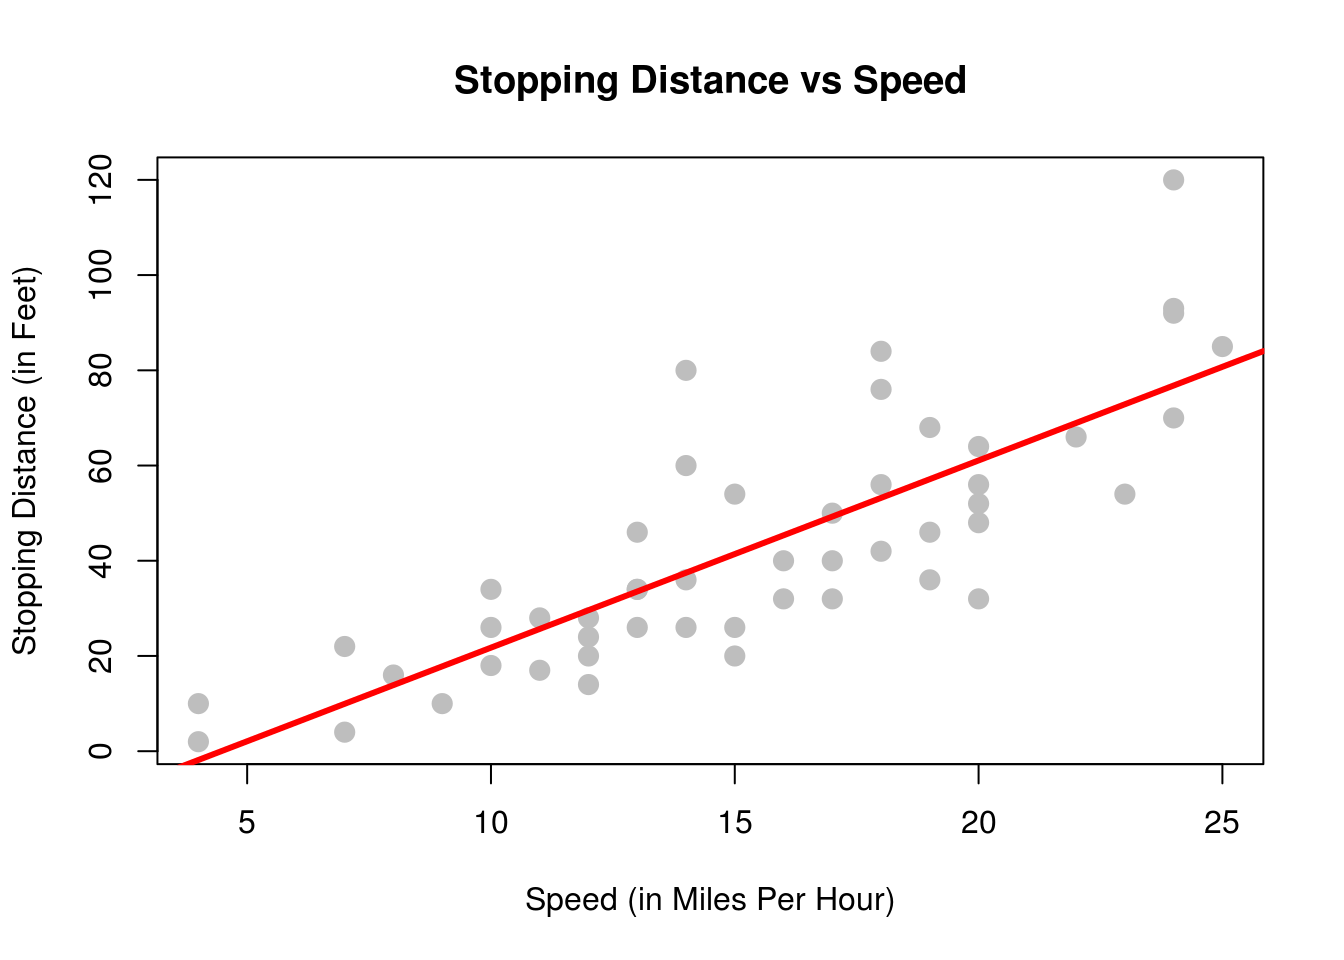
\includegraphics{ScPoEconometrics_files/figure-latex/cars-fig-1} 

}

\caption{A simple plot in R}\label{fig:cars-fig}
\end{figure}

\begin{Shaded}
\begin{Highlighting}[]
\KeywordTok{hist}\NormalTok{(}\KeywordTok{residuals}\NormalTok{(stop_dist_model),}\DataTypeTok{freq=}\OtherTok{FALSE}\NormalTok{)}
\KeywordTok{lines}\NormalTok{(}\KeywordTok{density}\NormalTok{(}\KeywordTok{residuals}\NormalTok{(stop_dist_model)),}\DataTypeTok{col=}\StringTok{'red'}\NormalTok{,}\DataTypeTok{lwd=}\DecValTok{3}\NormalTok{)}
\end{Highlighting}
\end{Shaded}

\begin{figure}

{\centering 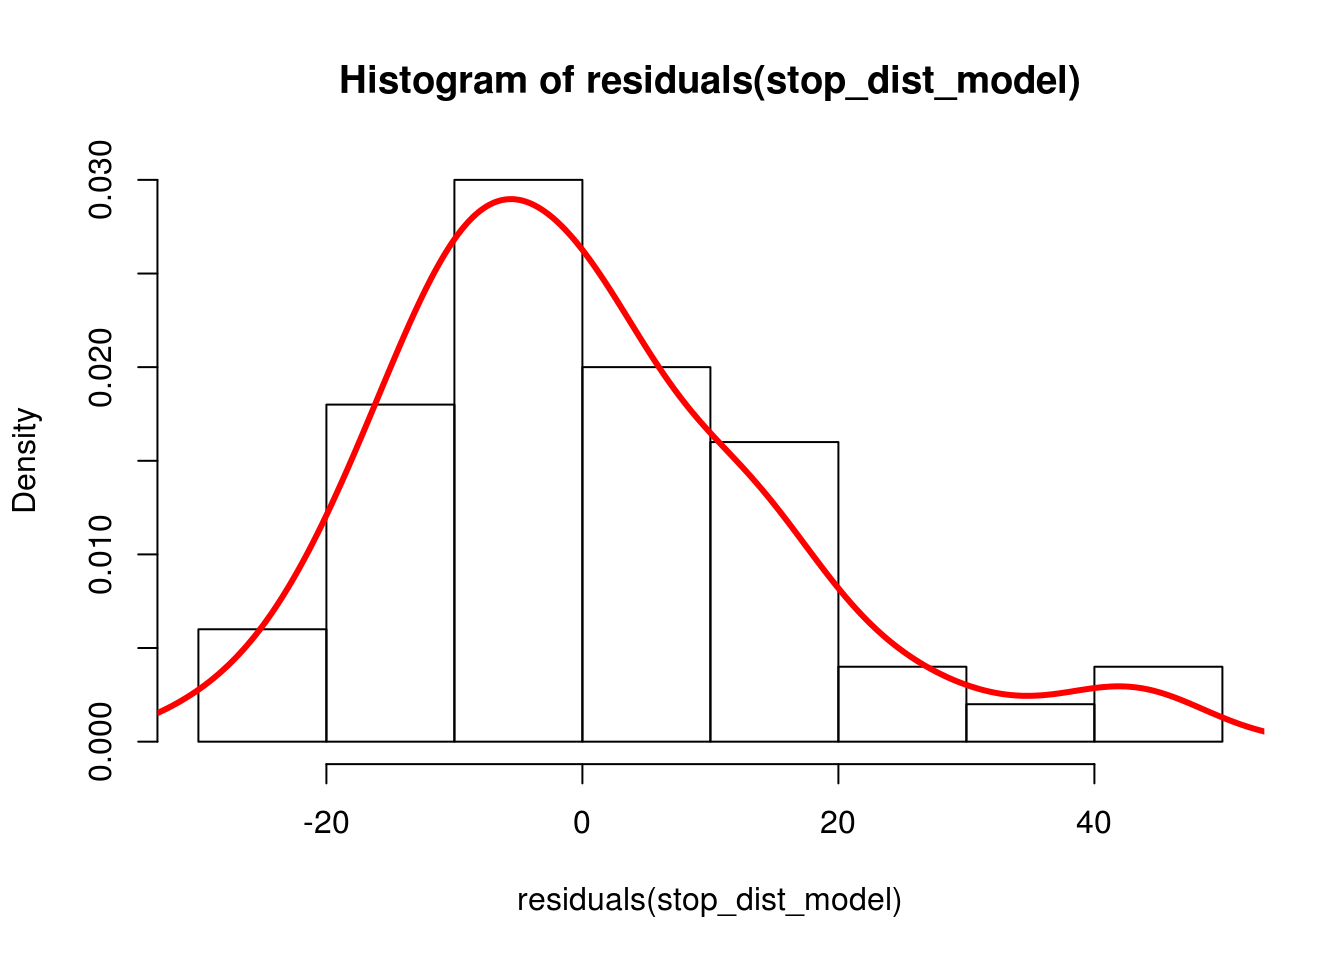
\includegraphics{ScPoEconometrics_files/figure-latex/hist-fig-1} 

}

\caption{what you were looking for}\label{fig:hist-fig}
\end{figure}

\section{Can do Math}\label{can-do-math}

\[
\begin{aligned}
R^2 &= \frac{\text{SSReg}}{\text{SST}} = \frac{\sum_{i=1}^{n}(\hat{y}_i - \bar{y})^2}{\sum_{i=1}^{n}(y_i - \bar{y})^2} \\[2.5ex]
    &= \frac{\text{SST} - \text{SSE}}{\text{SST}} = 1 - \frac{\text{SSE}}{\text{SST}} \\[2.5ex]
    &= 1 - \frac{\sum_{i=1}^{n}(y_i - \hat{y}_i)^2}{\sum_{i=1}^{n}(y_i - \bar{y})^2} = 
1 - \frac{\sum_{i = 1}^{n}e_i^2}{\sum_{i=1}^{n}(y_i - \bar{y})^2}
\end{aligned}
\]

But don't have to!

\chapter{Summarizing Data}\label{summarize-data}

We describe our methods in this chapter.

\chapter{Linear Regression}\label{linreg}

\begin{enumerate}
\def\labelenumi{\arabic{enumi}.}
\tightlist
\item
  linear regression - stop at R-squared

  \begin{enumerate}
  \def\labelenumii{\arabic{enumii}.}
  \tightlist
  \item
    different data: missing variable
  \item
    non-linear realtionship
  \end{enumerate}
\item
  scatter plot

  \begin{enumerate}
  \def\labelenumii{\arabic{enumii}.}
  \tightlist
  \item
    label observations
  \end{enumerate}
\item
  how do the data come to us? spreadsheet
\item
  approx link x and y by a line
\item
  OLS gives the best line for this

  \begin{enumerate}
  \def\labelenumii{\arabic{enumii}.}
  \tightlist
  \item
    \(y_i = a+b x_i\). find a,b s.t. dist is minimal
  \item
    write out sum of least-squares and call it MSE: u\_1 + u\_2 +
    \ldots{} / N
  \end{enumerate}
\item
  plot fitted values - see imperfect approximation
\item
  R-squared: goodness of fit / measure of goodness

  \begin{enumerate}
  \def\labelenumii{\arabic{enumii}.}
  \tightlist
  \item
    1 - sum of squared errors / SST
  \item
    how much of total variance is explained by the model?
  \end{enumerate}
\item
  regression on mean
\item
  How come there are residuals?

  \begin{enumerate}
  \def\labelenumii{\arabic{enumii}.}
  \tightlist
  \item
    measurement error?
  \item
    there is more to this than just x
  \item
    misspecification
  \end{enumerate}
\item
  There is statistical uncertainty about those estimates
\item
  plot a second data set with a less clear interpretation

  \begin{enumerate}
  \def\labelenumii{\arabic{enumii}.}
  \tightlist
  \item
    do you \emph{really} think there is a linear relationship?
  \item
    SE tells us whethe rwe really think this is a positive slope
  \item
    poor R2 and large standard error
  \item
    How \textbf{confident} are you about this relationship? Is there
    enought data?
  \item
    SE is ameasure of precision depending on N
  \end{enumerate}
\end{enumerate}

\chapter{Standard Errors}\label{std-errors}

\begin{enumerate}
\def\labelenumi{\arabic{enumi}.}
\tightlist
\item
  Standard Errors

  \begin{enumerate}
  \def\labelenumii{\arabic{enumii}.}
  \tightlist
  \item
    True data
  \item
    play with N and see how errors behave
  \end{enumerate}
\end{enumerate}

\chapter{Multiple Regression}\label{multiple-reg}

\begin{itemize}
\tightlist
\item
  Same as simple regression but more variables
\item
  income \textasciitilde{} age is not linear
\end{itemize}

\chapter{Categorial Variables: Dummies and
Interactions}\label{categorical-vars}

\begin{enumerate}
\def\labelenumi{\arabic{enumi}.}
\tightlist
\item
  if you only have educ categories, the estimate is like the conditional
  mean by educ
\item
  if you have too many categories you will have empty bins
\end{enumerate}

\chapter{Quantile Regression}\label{quantreg}

\begin{enumerate}
\def\labelenumi{\arabic{enumi}.}
\tightlist
\item
  before you were modelling the mean. the average link
\item
  now what happens to \textbf{outliers}? how robust is the mean to that
\item
  what about the entire distribution of this?
\end{enumerate}

\chapter{Panel Data}\label{panel-data}

\begin{itemize}
\tightlist
\item
  scanner data on breakfast cereals, \((Q_{it},D_{it})\)
\item
  why does D vary with Q
\item
  pos relation ship
\item
  don't observe the group identity!
\item
  unobserved het alpha is correlated with Q
\item
  within group estimator
\item
  what if you don't have panel data?
\end{itemize}

\chapter{Instrumental Variables}\label{IV}

\begin{enumerate}
\def\labelenumi{\arabic{enumi}.}
\tightlist
\item
  wage = educ
\item
  educ = ability
\item
  ols estimator captures your ability
\item
  you predict x by z and you only keep the variation that is in the
  error
\end{enumerate}

\chapter{Logit and Probit}\label{logit-probit}

\chapter{Principal Component Analysis}\label{pca}

\chapter{Notes}\label{notes}

this creates a library for the used R packages.

\section{Book usage}\label{book-usage}

You can label chapter and section titles using \texttt{\{\#label\}}
after them, e.g., we can reference Chapter \ref{intro}. If you do not
manually label them, there will be automatic labels anyway, e.g.,
Chapter \ref{linreg}.

Figures and tables with captions will be placed in \texttt{figure} and
\texttt{table} environments, respectively.

\begin{Shaded}
\begin{Highlighting}[]
\KeywordTok{par}\NormalTok{(}\DataTypeTok{mar =} \KeywordTok{c}\NormalTok{(}\DecValTok{4}\NormalTok{, }\DecValTok{4}\NormalTok{, .}\DecValTok{1}\NormalTok{, .}\DecValTok{1}\NormalTok{))}
\KeywordTok{plot}\NormalTok{(pressure, }\DataTypeTok{type =} \StringTok{'b'}\NormalTok{, }\DataTypeTok{pch =} \DecValTok{19}\NormalTok{)}
\end{Highlighting}
\end{Shaded}

\begin{figure}

{\centering 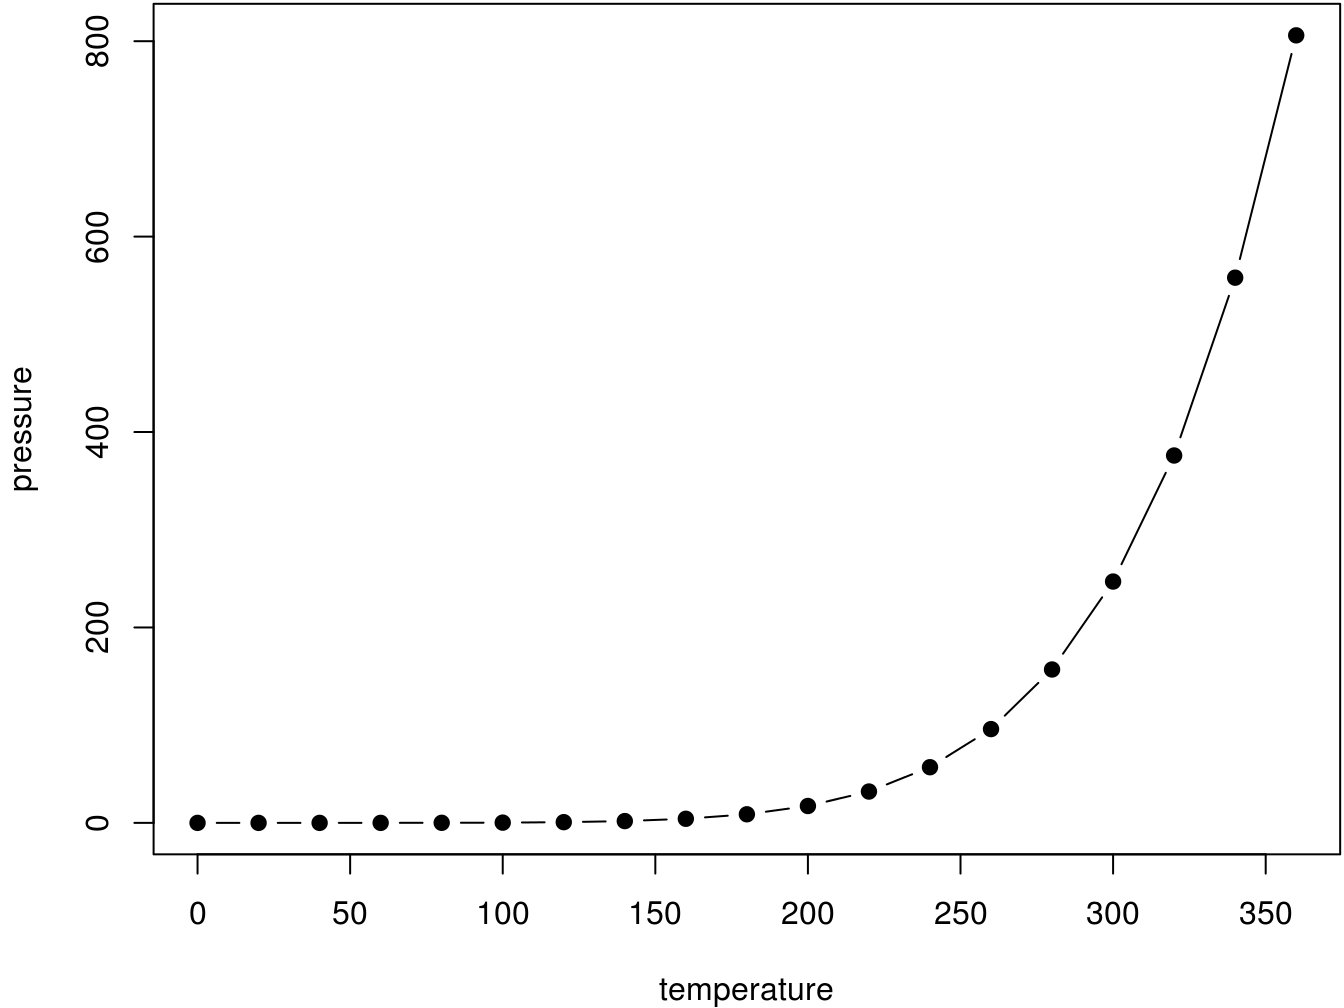
\includegraphics[width=0.8\linewidth]{ScPoEconometrics_files/figure-latex/nice-fig-1} 

}

\caption{Here is a nice figure!}\label{fig:nice-fig}
\end{figure}

Reference a figure by its code chunk label with the \texttt{fig:}
prefix, e.g., see Figure \ref{fig:nice-fig}. Similarly, you can
reference tables generated from \texttt{knitr::kable()}, e.g., see Table
\ref{tab:nice-tab}.

\begin{Shaded}
\begin{Highlighting}[]
\NormalTok{knitr}\OperatorTok{::}\KeywordTok{kable}\NormalTok{(}
  \KeywordTok{head}\NormalTok{(iris, }\DecValTok{20}\NormalTok{), }\DataTypeTok{caption =} \StringTok{'Here is a nice table!'}\NormalTok{,}
  \DataTypeTok{booktabs =} \OtherTok{TRUE}
\NormalTok{)}
\end{Highlighting}
\end{Shaded}

\begin{table}

\caption{\label{tab:nice-tab}Here is a nice table!}
\centering
\begin{tabular}[t]{rrrrl}
\toprule
Sepal.Length & Sepal.Width & Petal.Length & Petal.Width & Species\\
\midrule
5.1 & 3.5 & 1.4 & 0.2 & setosa\\
4.9 & 3.0 & 1.4 & 0.2 & setosa\\
4.7 & 3.2 & 1.3 & 0.2 & setosa\\
4.6 & 3.1 & 1.5 & 0.2 & setosa\\
5.0 & 3.6 & 1.4 & 0.2 & setosa\\
\addlinespace
5.4 & 3.9 & 1.7 & 0.4 & setosa\\
4.6 & 3.4 & 1.4 & 0.3 & setosa\\
5.0 & 3.4 & 1.5 & 0.2 & setosa\\
4.4 & 2.9 & 1.4 & 0.2 & setosa\\
4.9 & 3.1 & 1.5 & 0.1 & setosa\\
\addlinespace
5.4 & 3.7 & 1.5 & 0.2 & setosa\\
4.8 & 3.4 & 1.6 & 0.2 & setosa\\
4.8 & 3.0 & 1.4 & 0.1 & setosa\\
4.3 & 3.0 & 1.1 & 0.1 & setosa\\
5.8 & 4.0 & 1.2 & 0.2 & setosa\\
\addlinespace
5.7 & 4.4 & 1.5 & 0.4 & setosa\\
5.4 & 3.9 & 1.3 & 0.4 & setosa\\
5.1 & 3.5 & 1.4 & 0.3 & setosa\\
5.7 & 3.8 & 1.7 & 0.3 & setosa\\
5.1 & 3.8 & 1.5 & 0.3 & setosa\\
\bottomrule
\end{tabular}
\end{table}

You can write citations, too. For example, we are using the
\textbf{bookdown} package \citep{R-bookdown} in this sample book, which
was built on top of R Markdown and \textbf{knitr} \citep{xie2015}.

\bibliography{book.bib,packages.bib}


\end{document}
